\section*{הקדמה}
\begin{displayquote}
אלגוריתם הוא דרך שיטתית (כלומר כזו שצעדיה מוגדרים היטב) לביצוע של משימה מסוימת, 
במספר סופי של צעדים.
\end{displayquote}
\leftline{\textenglish{---} \textit{ויקיפדיה}}
המושג אלגוריתם אינו חדש עבורנו, ראינו ומימשנו כבר אלגוריתמים בקורס מבוא למדעי המחשב, 
מבוא לתכנות מערכות ומבני נתונים.
\subsection*{חשיבות הקורס}
בתעשייה - בעיות שמצריכות פתרון אלגוריתמי צצות במגוון תחומים. על פי
\textenglish{glassdoor}, 
מפתח אלגוריתמים מרוויח 20 אחוז יותר מאשר מהנדס תוכנה.
\\
במחקר האקדמי - חלק עיקרי של המחקר האקדמי הוא בפיתוח וניתוח אלגוריתמים.
\subsection*{חומר הקורס}
בקורס נלמד מגוון אלגוריתמים שעל פי רוב נחשבים לבסיס בתחום האלגוריתמים.
הרוב המוחלט של האלגוריתמים שנלמד בקורס הם אלגוריתמים על גרפים 
וזאת מכיוון שגרפים הוכיחו את עצמם ככלי מאוד חזק בייצוג מגוון רחב של בעיות.
לחלק מהאלגוריתמים שימושים ברורים (מסלול קצר ביותר, עצי הופמן), 
חלק מהאלגוריתמים מהווים פתרון למגוון גדול של בעיות שניתנות לייצוג בצורה מסוימת (זרימה), 
וחלק מהאלגוריתמים מהווים בסיס לפיתוח אלגוריתמים מורכבים יותר (%
\textenglish{BFS},
\textenglish{DFS}, 
עץ פורש).
מעבר לזה נלמד טכניקות (פשוטות יחסית) כלליות לפיתוח אלגוריתמים.
\section*{אלגוריתמי חיפוש בגרפים}
\begin{example}
רוצים למצוא (ולהדפיס) את כל קבצי התמונות ששמורות על הכונן הקשיח.
\end{example}
למשל עבור:
\begin{center}
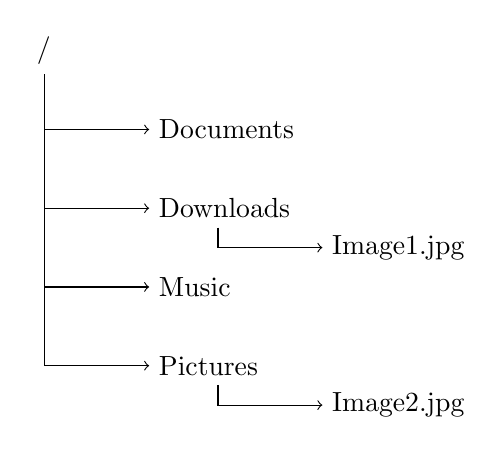
\begin{tikzpicture}[every node/.style={
	rectangle
%	, minimum width=1.5cm
%	, draw
	, text width=1.5cm
	, x=2.2cm
}, ->]

\node[text width=2mm](0) at(0,1) {/};
\foreach [count=\i] \x \y \name in {
	1/0/Documents
	, 1/-1/Downloads
	, 1/-2/Music
	, 1/-3/Pictures
	, 2/-1.5/Image1.jpg
	, 2/-3.5/Image2.jpg	
}{
	\node(\i) at(\x, \y) {\name};
}

\foreach \i in {1,...,4}{
	\draw (0) |- (\i);
}
\draw (2) |- (5);
\draw (4) |- (6);

\end{tikzpicture}
\end{center}

כיצד עלינו לסרוק (לחפש) את מערכת הקבצים ? 
\begin{enumerate}
\item
במידה ורוצים להדפיס את (הנתיב המלא של) הקבצים בסדר לקסיקוגרפי ?
\item
במידה ורוצים להדפיס קבצים לפי העומק שלהם (מספר תיקיות) ?
\end{enumerate}
נשים לב שאפשר לייצג את מערכת הקבצים באמצעות גרף מכוון (ברוב מערכות הקבצים עץ אינו ייצוג מספק)
ולכן נעביר את הדיון שלנו לחיפוש בגרפים.

\subsection*{ייצוג גרפים}
קיימים שני ייצוגים סטנדרטים של גרפים (מכוונים או לא):
\begin{enumerate}
\item
על ידי מטריצת שכנויות
\item
על ידי רשימת שכנויות
\end{enumerate}
אם לא מצוין אחרת, נניח שהגרף מיוצג על ידי רשימת שכנויות.



\subsection*{אלגוריתם כללי}
\textbf{קלט:}
גרף $G$ (מכוון או לא) וצומת מקור $s$.
\\
\textbf{מטרה:}
למצוא תת עץ שפורש את כל הצמתים שישיגים מ-$s$.
\begin{enumerate}
\item 
אתחול:
$T \leftarrow \emptyset$, 
$U \leftarrow \{s\}$
ולכל 
$v \in V$
מציבים 
$p(v) \leftarrow \text{nil}$
\item
כל עוד יש קשת
$uv$
עם
$u \in U, v \notin U$
	\begin{enumerate}
	\item
	$U \leftarrow U \cup \{v\}$,
	$T \leftarrow T \cup \{uv\}$,
	$p(v) \leftarrow u$
	\end{enumerate}
\end{enumerate}

\begin{observation}
בסיום ריצת ריצת האלגוריתם
$U$
מכילה את כל הצמתים הישיגים מ-$s$
\end{observation}
\begin{proof}
בשלילה, בוחרים מסלול מ-$s$ לצומת $v$ שלא נכנס ל-%
$U$
ומסתכלים על הצומת הראשון במסלול שלא נכנס.
\end{proof}
\begin{observation}
בכל שלב בריצת האלגוריתם
$T$
עץ קשיר
\end{observation}
\begin{proof}
באינדוקציה על צעד האלגוריתם.
\end{proof}
\begin{theorem}
בסיום ריצת האלגוריתם הכללי $T$ הוא עץ שפורש את כל הצמתים הישיגים מ-$s$
\end{theorem}





\subsection*{BFS}
\textbf{קלט:}
גרף $G$ (מכוון או לא) וצומת מקור $s$.
\\
\textbf{מטרה:}
למצוא תת עץ, $T$, שפורש את כל הצמתים שישיגים מ-$s$ כך שלכל צומת 
$v \in V$
מתקיים
$dist_T(s, v) = dist_G(s, v)$.
\\
למשל:
\begin{center}
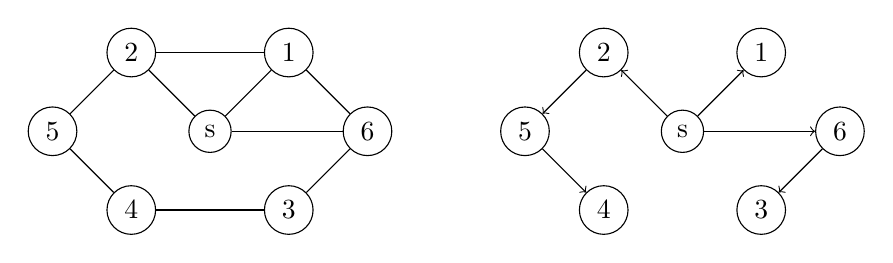
\begin{tikzpicture}[every node/.style={circle, draw, minimum width=5mm}]


\node(s) at(0,0) {s};
\foreach [count=\i] \x\y in {
	1/1
	,-1/1
	,1/-1
	,-1/-1
	,-2/0
	,2/0	
}{
	\node(\i) at(\x,\y) {\i};
}

\foreach \u \v in {
s/1%
,s/6%
,6/3%
,1/6%
,s/2%
,1/2%
,2/5%
,5/4%
,4/3%
}{
	\draw (\u) -- (\v);
}

\begin{scope}[xshift=6cm]
\node(s) at(0,0) {s};
\foreach [count=\i] \x\y in {
	1/1
	,-1/1
	,1/-1
	,-1/-1
	,-2/0
	,2/0	
}{
	\node(\i) at(\x,\y) {\i};
}

\foreach \u \v in {
s/1%
,s/6%
,6/3%
,s/2%
,2/5%
,5/4%
}{
	\draw[->] (\u) -- (\v);
}
\end{scope}

\end{tikzpicture}
\end{center}

\begin{enumerate}
\item
אתחול:
$U \leftarrow \{s\}, T \leftarrow \emptyset, i \leftarrow 0$, 
לכל 
$v \in V$
מציבים
$p(v) \leftarrow nil, d(v) \leftarrow \infty$
\item
$d(s) \leftarrow 0$
\item
עבור כל קשת 
$uv$
כך ש-%
$d(u) = i, v \notin U$
	\begin{enumerate}
	\item
	$U \leftarrow U \cup \{v\}, T \leftarrow T \cup \{uv\}$
	\item
	$p(v) = u, d(v) = i + 1$
	\end{enumerate}
\item
$i \leftarrow i+1$
\end{enumerate}









\subsection*{DFS}

\begin{example}[פאזל הזזה]
נתון לוח משחק בגודל 
$n \times m$
על הלוח 
$nm - 1$
חלקים ממוספרים מ-1 עד 
$nm - 1$
ומשבצת ריקה.
נתון סידור ראשוני של החלקים ואנו רוצים לסדר את החלקים לפי הסדר 
כך שבכל שלב מותר לנו להזיז את אחד החלקים ששכנים למשבצת הריקה אל המשבצת הריקה.
\end{example}
למשל עבור
$n = m = 3$:
\begin{center}
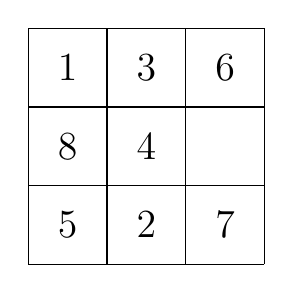
\begin{tikzpicture}
\draw (0,0) grid (3,3);

\begin{scope}[xshift=.5cm, yshift=.5cm, font=\Large]
\foreach \x \y \i in {0/0/5, 1/0/2, 2/0/7, 0/1/8, 1/1/4, 0/2/1, 1/2/3, 2/2/6}{
	\node at(\x, \y) {\i};
}
\end{scope}

\end{tikzpicture}
\end{center}


הציעו אלגוריתם לפתרון הבעיה.
